\documentclass[border=5pt]{standalone}
\usepackage{tikz}
\usepackage{tikz-3dplot}
\usetikzlibrary{arrows.meta, 3d, perspective, calc}
\usepackage{amsmath}
\begin{document}
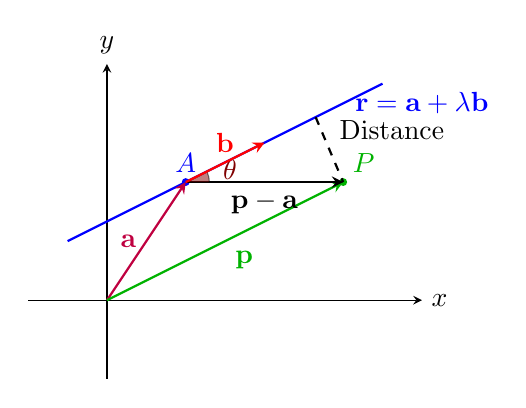
\begin{tikzpicture}[scale=1, >=stealth]
    % Coordinate system
    \draw[->] (-1,0) -- (4,0) node[right]{$x$};
    \draw[->] (0,-1) -- (0,3) node[above]{$y$};

    % Point A
    \coordinate (A) at (1,1.5);
    \fill[blue] (A) circle (0.05) node[above] {$A$};

    % Line
    \draw[thick, blue, -] (-0.5,0.75) -- (3.5,2.75);

    % Position vector to A
    \draw[->,thick,purple] (0,0) -- (A) node[midway,left] {$\mathbf{a}$};

    % Generic position vector r
    \coordinate (P) at (3,1.5);
    \fill[green!70!black] (P) circle (0.05) node[above right] {$P$};
    \draw[->,thick,green!70!black] (0,0) -- (P) node[midway,below right] {$\mathbf{p}$};

    % r-a vector
    \draw[->,thick] (A) -- (P) node[midway,below] {$\mathbf{p}-\mathbf{a}$};

    \begin{scope}
        \path[clip] (A) -- (P) -- ($(A)+(1,0.5)$);
        \fill[red!50!black, opacity=0.5, draw=black] (A) circle (3mm);
    \end{scope}
    \node[right, red!50!black] at (1.35,1.65) {$\theta$};

    \draw[thick, dashed] ($(A)+(1.65,0.825)$) -- (P) node[midway, above right] {Distance};

    % Vector b
    \draw[->,thick,red] (A) -- ($(A)+(1,0.5)$) node[midway, above] {$\mathbf{b}$};

    % Label the line equation
    \node[blue] at (4,2.5) {$\mathbf{r} = \mathbf{a} + \lambda\mathbf{b}$};
\end{tikzpicture}
\end{document}
